\documentclass[11pt,twocolumn]{article}

\usepackage{epsfig}
\usepackage{graphicx}
\usepackage{graphpap}
\usepackage{amsmath}
\usepackage[utf8]{inputenc}
\usepackage[spanish]{babel}

\topmargin -2.5 cm
\textheight 9.5in
\oddsidemargin -1cm
%\evensidemargin -1cm
\textwidth 18cm
%opening
\title{}
\author{}
\date{}

\newcommand{\abre}{\textquestiondown}

\begin{document}
\pagestyle{empty}
\sffamily
\twocolumn[Física de Campos. Taller 2.1: \textbf{Campo y potencial gravitacional}

\hrulefill 
]

\footnote{Algunas de las figuras han sido tomadas en su gran mayoría de Physics For Scientist and Engineers 6E By Serway and Jewett.}

\begin{enumerate}
%ejercicio
\item Una barra de longitud $l$ tiene una masa por unidad de longitud $\lambda$ y una masa total $m$. Calcule el campo gravitacional $\vec{g}$ y el potencial gravitacional en un punto $P$ a lo largo del eje de la barra a una distancia $a$ de uno de los extremos.
{
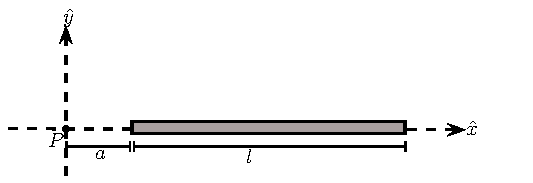
\includegraphics[scale=1.0]{barra}
}
\begin{displaymath}
\vec{g}=\dfrac{G m}{a(a+l)} \hat{i}
\end{displaymath}
\small{Note que para $a\gg l$ la barra se comporta como una masa puntual.} 

%ejercicio
\item Un anillo de radio $R$ tiene una masa $m$ uniformemente distribuida. Calcule el campo y el potencial gravitacional a una distancia $x$ a lo largo del eje del anillo.
%{
%\begin{center}
%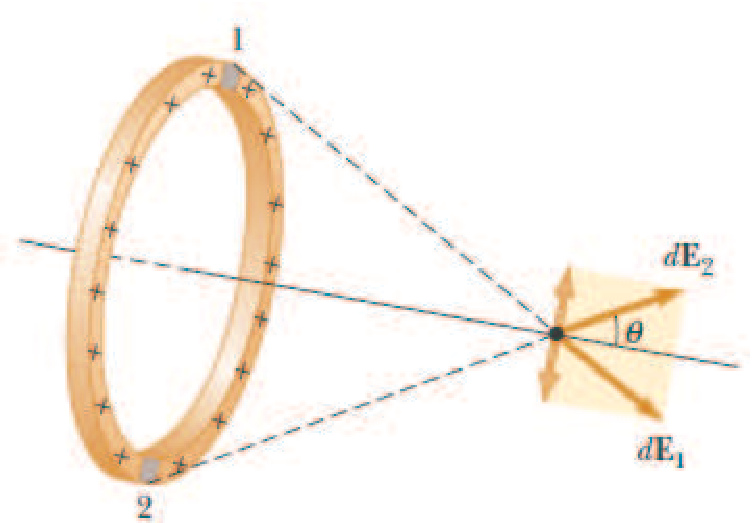
\includegraphics[scale=0.3]{anillo}
%\end{center}
%}
\begin{displaymath}
\vec{g}=-\dfrac{G m x}{(R^2+x^2)^{3/2}} \hat{i} \hspace{0.7 cm} V=-\dfrac{G m}{\sqrt{x^2 +R^2}}
\end{displaymath}
\small{Note que para $x\gg R$ el anillo se comporta como una masa puntual $m$.} 

%ejercicio
\item Un disco de radio $R$ tiene una masa uniforme por unidad de área $\sigma$. Calcule el campo y el potencial gravitacional a lo largo del eje del disco a una distancia $x$ de su centro.
{
\begin{center}
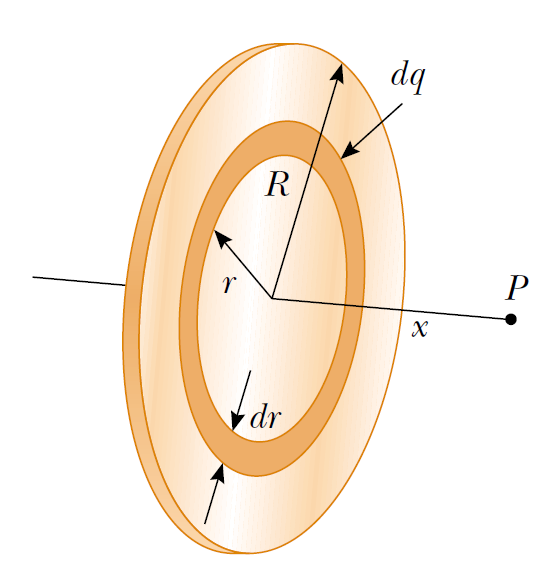
\includegraphics[scale=0.2]{disco}
\end{center}
}
\begin{displaymath}
\vec{g}=-2\pi G \sigma \Big(1-\dfrac{x}{(x^2+R^2)^{1/2}}\Big)\hat{i}
\end{displaymath}
\small{Note que para $x\gg a$ el disco se comporta como una masa puntual $m$.} 

%ejercicio
\item Una esfera de radio $a$ tiene una masa $m$ distribuida uniformemente. 
\begin{enumerate}
\item Calcule el campo y el potencial gravitacional en un punto interno ($r \leq a$).  
\item Calcule el campo y el potencial gravitacional en un punto externo ($r\geq a$).  
\end{enumerate}
{
\begin{center}
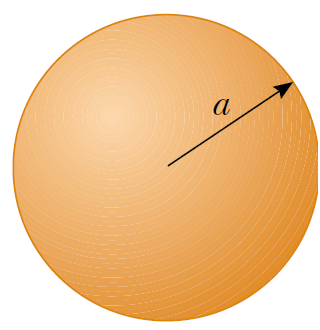
\includegraphics[scale=0.2]{esfera}
\end{center}
}
\begin{displaymath}
\vec{g}=-G\dfrac{m}{r^2}\hat{u_{r}} \hspace{0.2 cm} (r \geq a) \hspace{0.6 cm} \vec{g}=-G\dfrac{m r}{a^3}\hat{u_{r}} \hspace{0.2 cm} (r \leq a)
\end{displaymath}
\begin{displaymath}
V=-G\dfrac{m}{r} \hspace{0.2 cm} (r\geq a) \hspace{0.6 cm} V=-\dfrac{G m}{2a}\Big(3-\dfrac{r^2}{a^2}\Big) \hspace{0.2 cm} (r\leq a)
\end{displaymath}


%ejercicio 5
\item Considere un disco hueco de radio exterior $R_{1}$ e interior $R_{2}$ y masa $m$ uniformemente distribuida. 
\begin{enumerate}
\item Halle el campo y el potencial gravitacional en un punto $P$ a lo largo del eje del disco.
\begin{displaymath}
\vec{g}=-\dfrac{2Gm}{(R_{1}^2 -R_{2}^2)}\Big[\dfrac{z}{\sqrt{R_{1}^2 +z^2}}- \dfrac{z}{\sqrt{R_{2}^2 +z^2}}\Big]\hat{k}
\end{displaymath}
\begin{displaymath}
V= -\dfrac{2Gm}{(R_{1}^2 -R_{2}^2)}\Big[\sqrt{R_{1}^2 + z^2} - \sqrt{R_{2}^2 +z^2}\Big]
\end{displaymath}
\item Analize el caso cuando $R_{1} \to 0$ (dese cuenta que en ese caso se tiene un disco). Analize el caso cuando $R_{1} \to 0$ y $R_{2} \to \infty $ (dese cuenta que en este caso se tiene un plano infinito).
\end{enumerate}

%ejercicio 6
\item *Considere dos barras uniformes de longitud $l$ y masa $m$ colocadas a lo largo de la misma línea y que tienen sus puntos más cercanos separados una distancia $d$. Muestre que la fuerza gravitacional mutua entre las dos barras es:
\begin{displaymath}
F_{g}= G\dfrac{m^2}{l^2} \ln \Big[\dfrac{(l+d)^2}{d(2l+d)}\Big]
\end{displaymath}  

%ejercicio
\item Una varilla de masa $m$ es doblada en forma de semicírculo de radio $R$. Calcule el campo y el potencial gravitacional en el centro del semicírculo.
\begin{displaymath}
\vec{g}=-\dfrac{2Gm}{\pi}\dfrac{1}{R^2} \hat{j} \hspace{1.0 cm} V=\cdots
\end{displaymath} 
{
\begin{center}
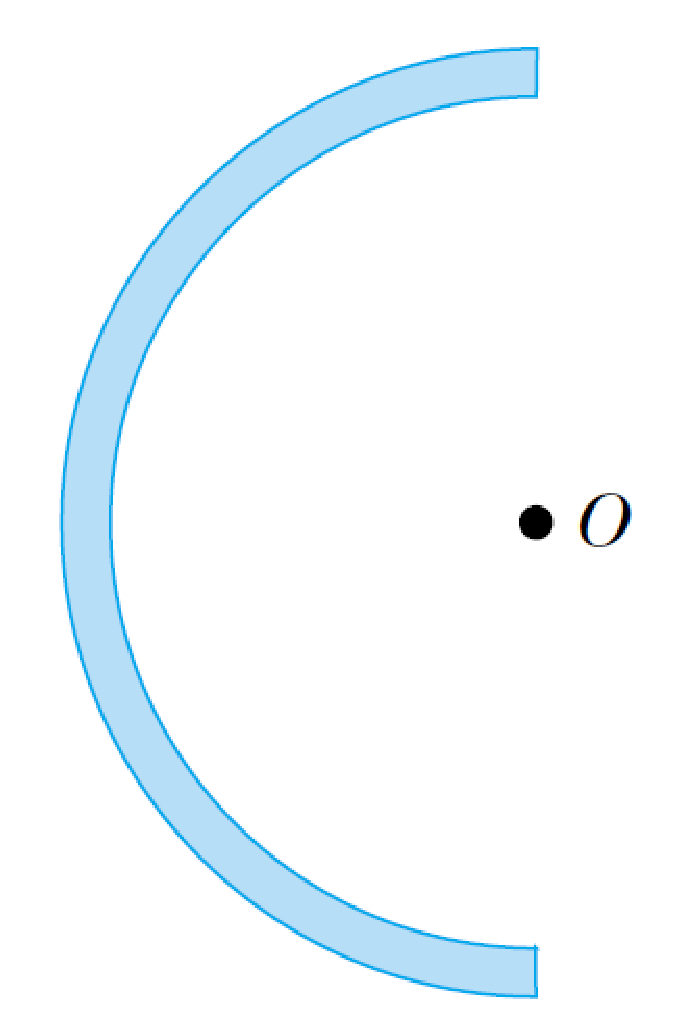
\includegraphics[scale=0.2, angle=-90]{media-barilla}
\end{center}
}

%ejercicio
\item *Calcule el campo y el potencial gravitacional de una varilla finita de longitud $l$ y densidad de masa $\lambda$ a lo largo de un eje perpendicular a la varilla y que pase por el centro de la misma.
\begin{displaymath}
\vec{g}=\cdots \hat{j} \hspace{1.0 cm} V=\cdots
\end{displaymath}
{
\begin{center}
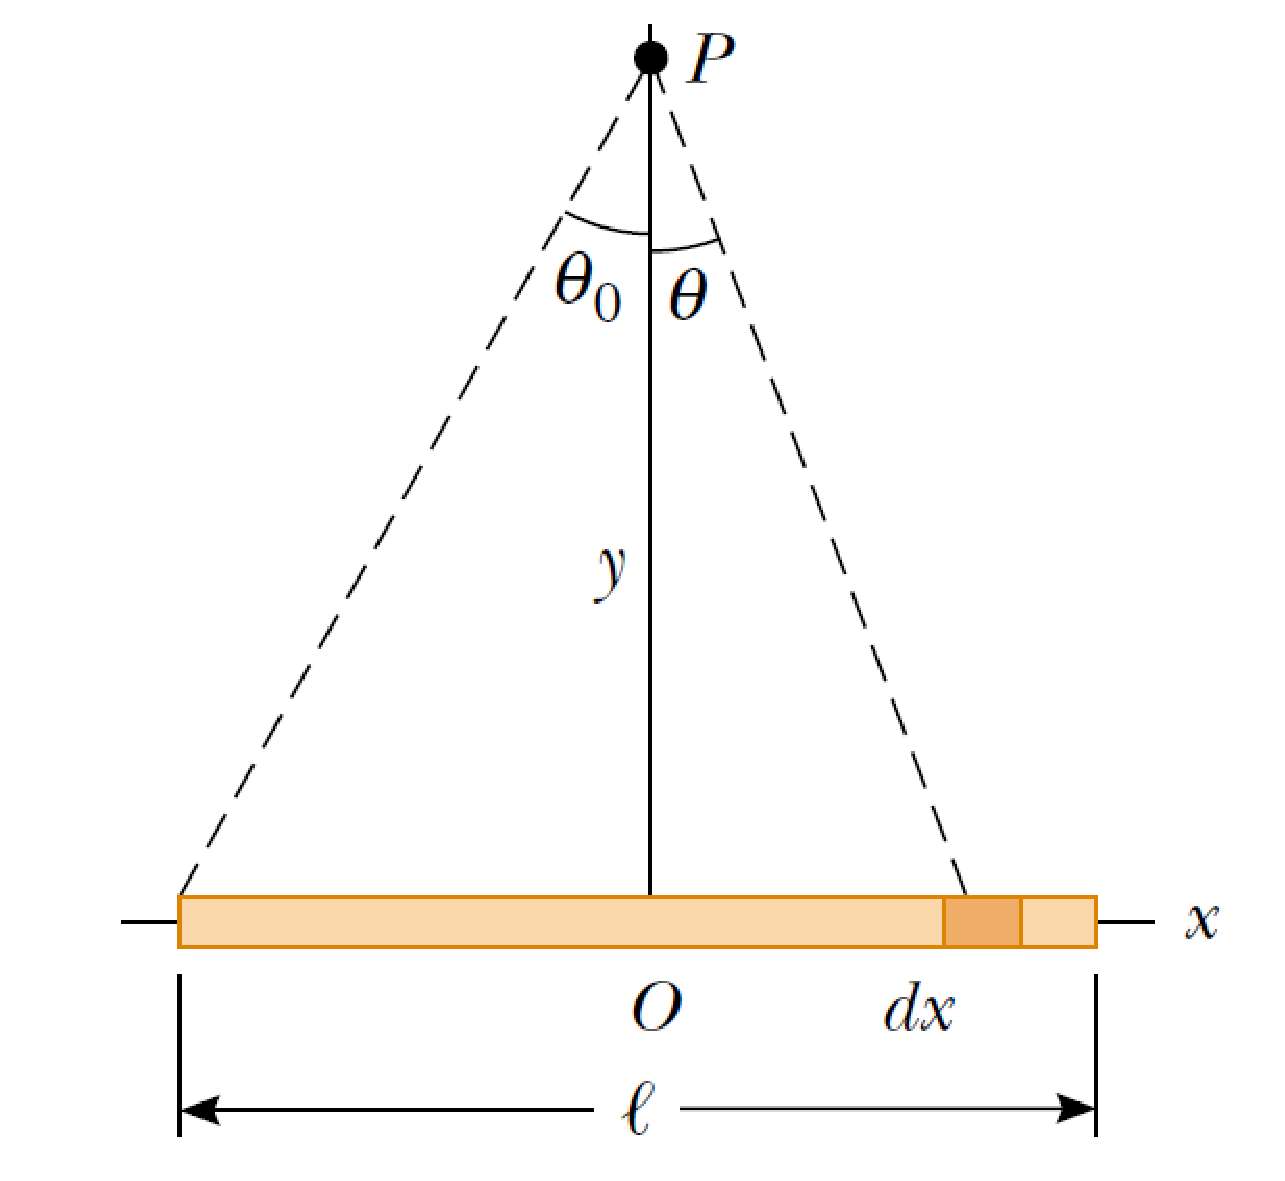
\includegraphics[scale=0.25]{varilla-finita}
\end{center}
}

%ejercicio
\item Calcule el campo y el potencial gravitacional de una varilla infinita de densidad de masa $\lambda$.
\begin{displaymath}
\vec{g}=-\dfrac{2G\lambda}{r}\hat{u_{r}} \hspace{1.0 cm} V=\cdots
\end{displaymath}

%ejercicio
\item *Calcule el campo y el potencial gravitacional de un plano infinito de densidad de masa superficial $\sigma$.
\begin{displaymath}
\vec{g}=-2\pi G\sigma \hat{k} \hspace{1.0 cm} V=2\pi G \sigma z
\end{displaymath}


\end{enumerate}
\end{document}
